\chapter{Design}\label{ch:design}
In the following chapter we examine the design of this system.
To do so, we will design and describe prototypes for the system to be used when designing the front end.
A class diagram will be constructed to define the parts of the system, as well as an architecture diagram to define how the different components interact.
A choice of framework has to be made for the front end, and this will be described in this chapter, and an introduction to the chosen framework will be written.
We discuss the API design, and the structure of the database through an entity-relationship diagram.
Finally, we will take a look at the different methods for recommending items to users.
\section{Prototypes}
To get a clear view of how the different pages will look and catch any early potential design problems, we have created prototypes for each of the different pages. 
We will use these to make the implementation of the different pages easier to ensure that we have a consistent design throughout the system. 
The prototypes will not serve as an exact vision of how the pages will look but will instead serve as a guideline to how the page should be set up.
In this section, we will look at some of the more interesting prototypes where we have had to make some design choices.
\begin{figure}[H]
    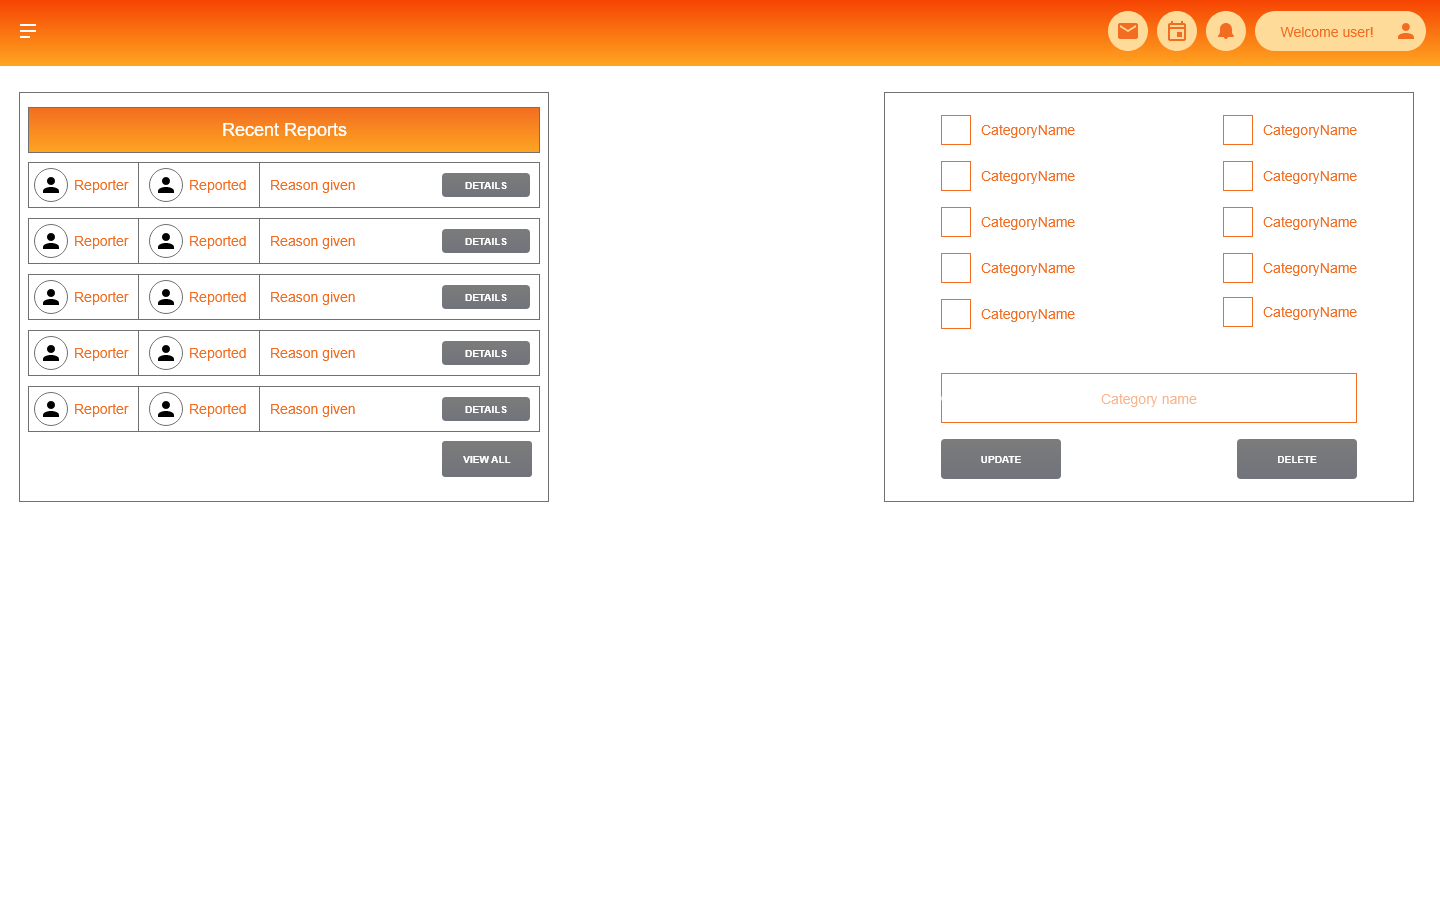
\includegraphics[width=\linewidth]{/prototypes/admin-dashboard.png}
     \caption{Shows the admin dashboard for admins that are logged into the system}
     \label{fig:admin-dashboard}
 \end{figure}
The admin dashboard gives the admin an overview of the recently reported tutors and the different categories. 
The admin needs to see tutor reports since they are the ones that will handle them and decide if a tutor should be banned. 
Admins are also in charge of the different teaching categories, and therefore, they need to have an overview of the current ones and also be able to add new categories.
We also have a top bar that is used on every page for when the user is logged in. It shows a couple of different icons where the user can go to the inbox, the calendar, or the user's own page. 
It will also show notifications for when different events related to the user happen in the system. 
On the far left side of the top bar, we will place a logo, which will lead to the landing page.
\begin{figure}[H]
   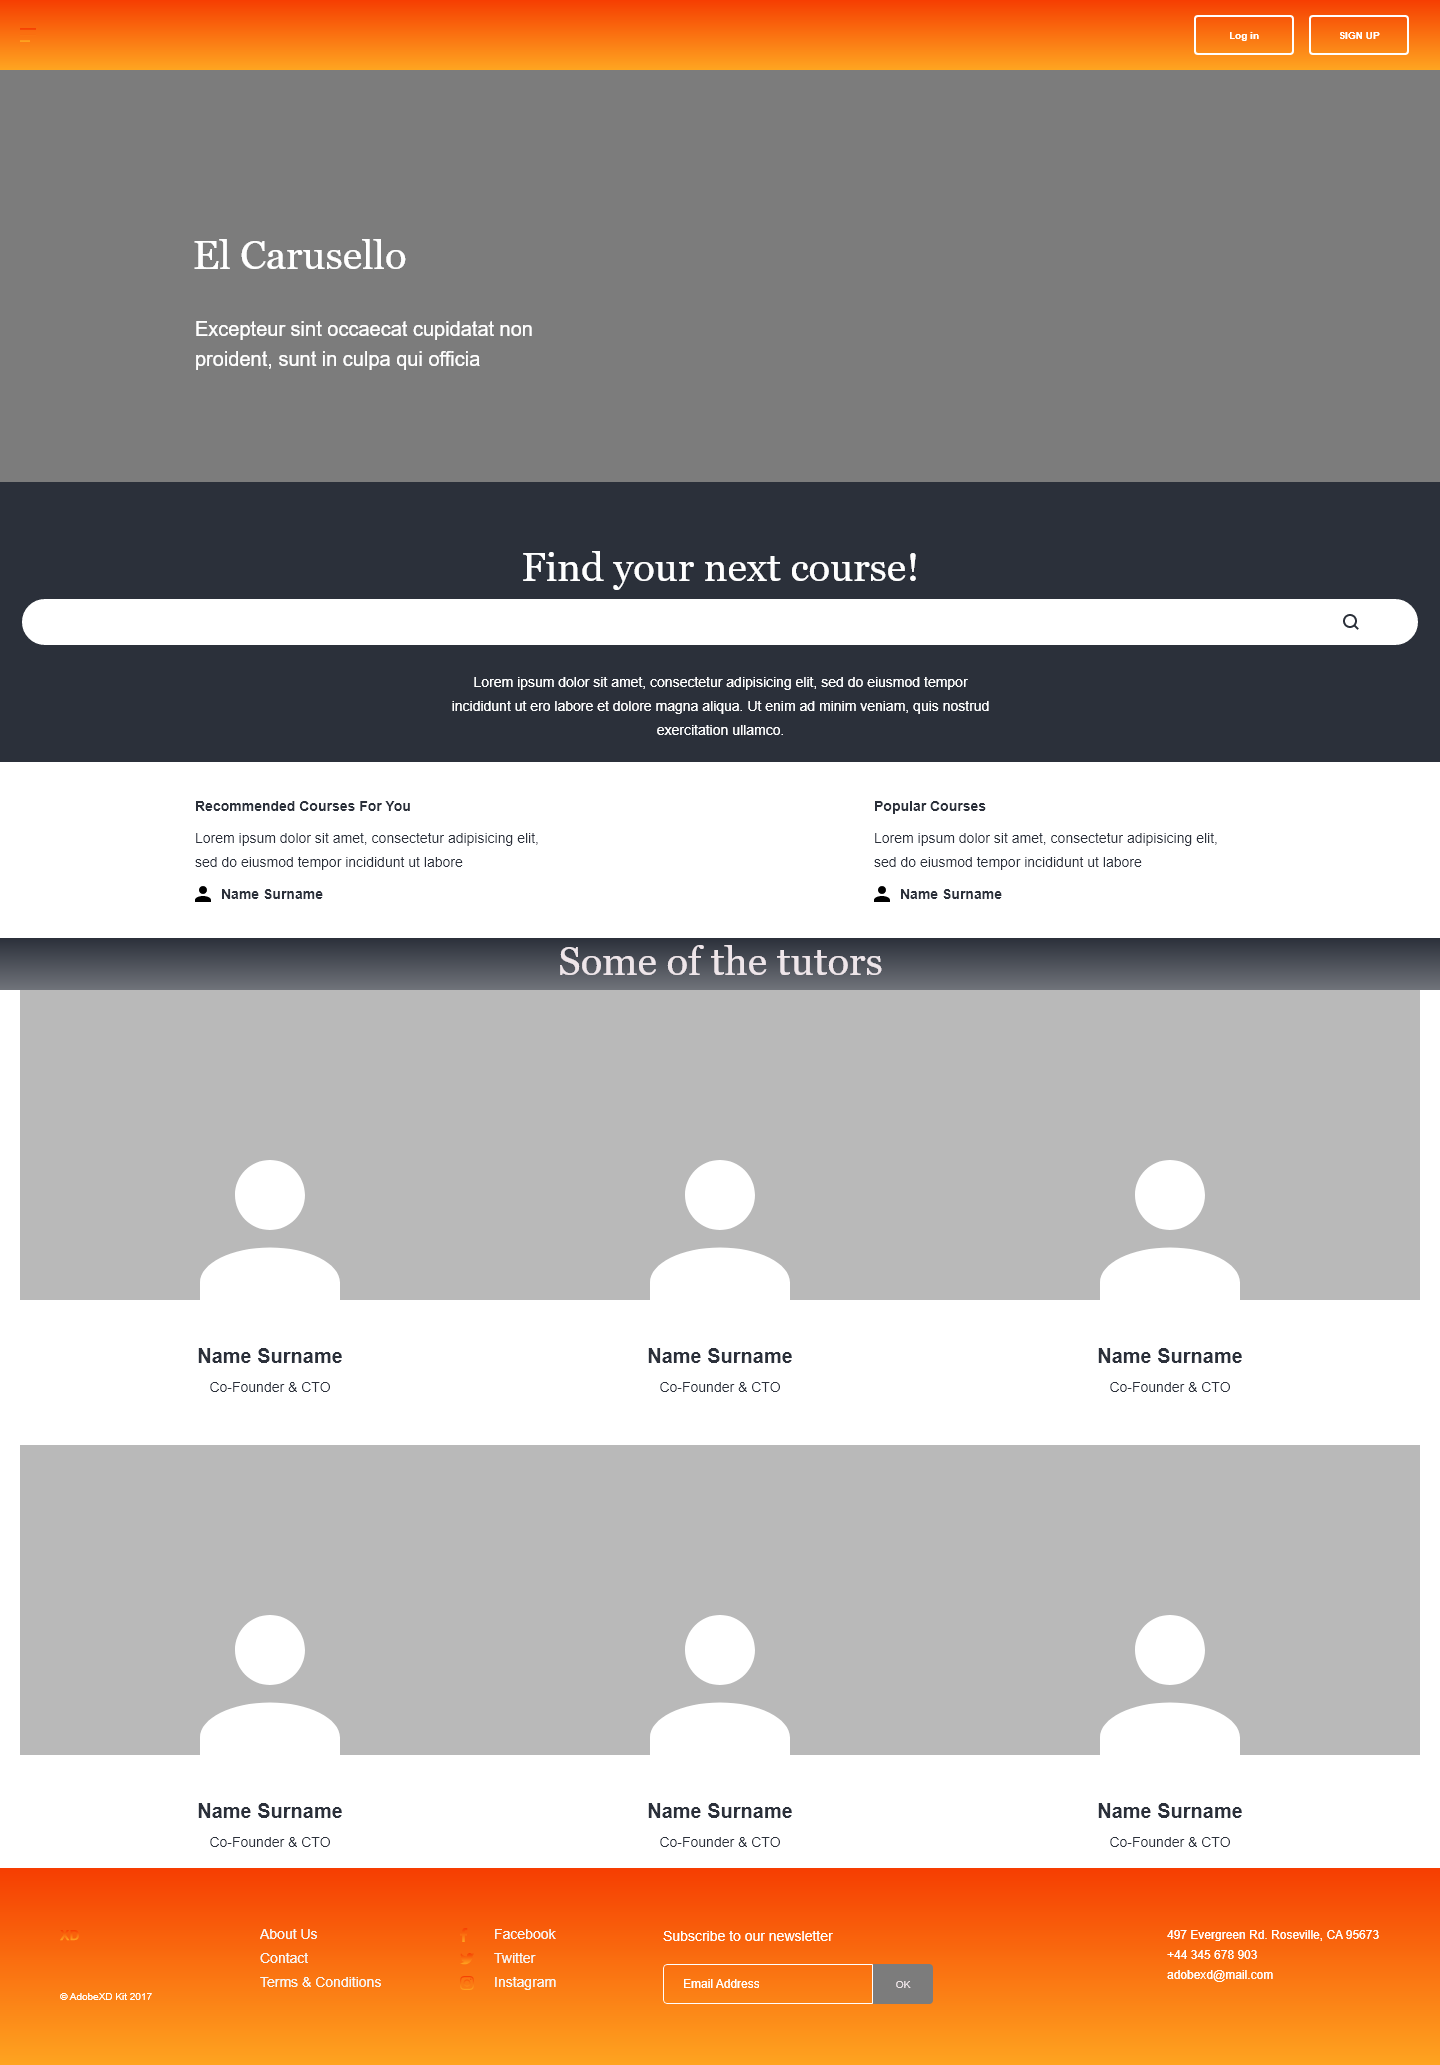
\includegraphics[width=\linewidth, scale=0.5]{/prototypes/landing-page.png}
    \caption{The landing page for the system}
    \label{fig:landing-page}
\end{figure}
The landing page is the first page that the users of the system will see, and thus it is important that this page shows some interesting content. 
This page can be accessed both with and without being logged in. 
We have a top bar that changes depending on if the user is logged in or not. 
At the top of the landing page, we will have a carousel that shows some interesting images.
Underneath, we have included a search functionality to find a course or a specific tutor. 
The user should be able to search for both tutors and courses. 
Finally, there will be some recommendations for the user, which will suggest specific tutors based on their profile information and previously taken courses.

 \begin{figure}[H]
    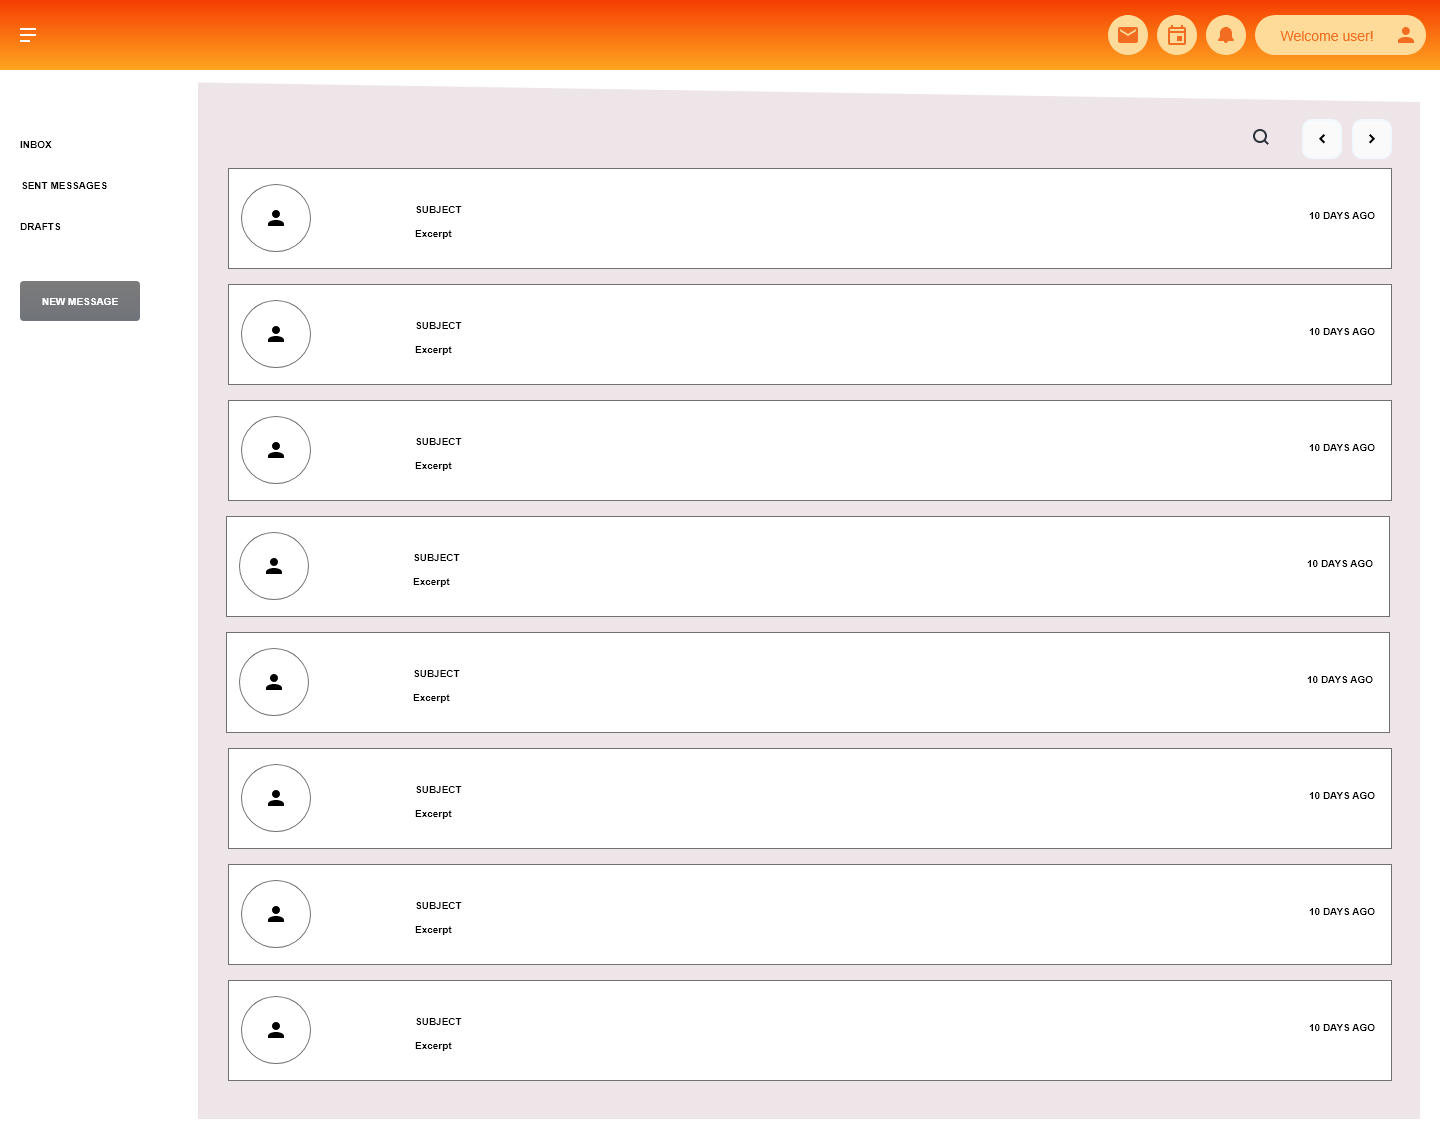
\includegraphics[width=\linewidth]{/prototypes/inbox.png}
     \caption{The inbox for the messaging component in the system}
     \label{fig:inbox}
 \end{figure}
When the user clicks the message icon in the top bar they will be redirected to the inbox page. Here they can view their recent messages. 
We considered including a search functionality to find specific messages but ultimately did not add it to the prototypes. 
The most recently received messages should be shown on the top of the list, so they are easy to find. 
When a message is received, the topbar should also show a notification for this. 
There should also be an indicator that shows if the user has unread messages. 
The user can click a button on the left side of the page to start writing a new message. 


 \begin{figure}[H]
    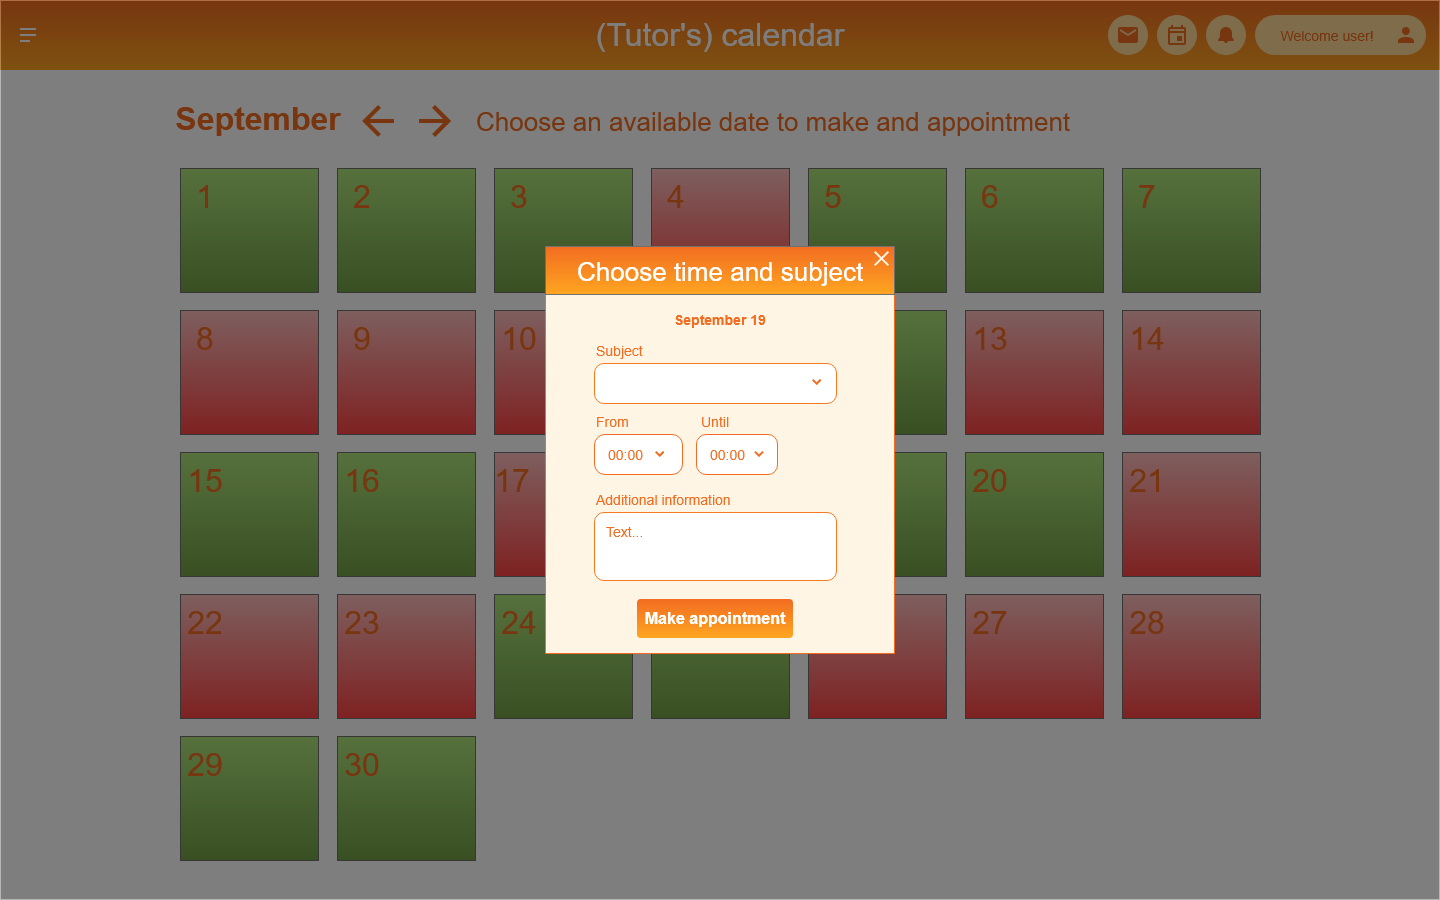
\includegraphics[width=\linewidth]{/prototypes/make-appointment.png}
     \caption{Page that shows a tutor's calendar where the student can request an appointment}
     \label{fig:make-appointment}
 \end{figure}
 This page is the tutor's calendar from a student's point of view. 
 The student is able to browse the tutor's calendar and look for a date where the tutor is available, shown as the color green. 
 The student then clicks the desired date, and the popup window will show. 
 Here they can specify the subject they wish to be taught and the timeslot as well as additional information. 
 They can only choose one of the tutors available subjects, and the timeslot should comply with the tutor's availability. 
 The tutor also needs to choose what time they are available prior to this.
 When the student makes the appointment, they will be sent to a payment page, and a request will be sent to the tutor, which they can either accept or deny.
 However, the money will not be withdrawn from the students account until the tutor has approved the appointment.

 \begin{figure}[H]
    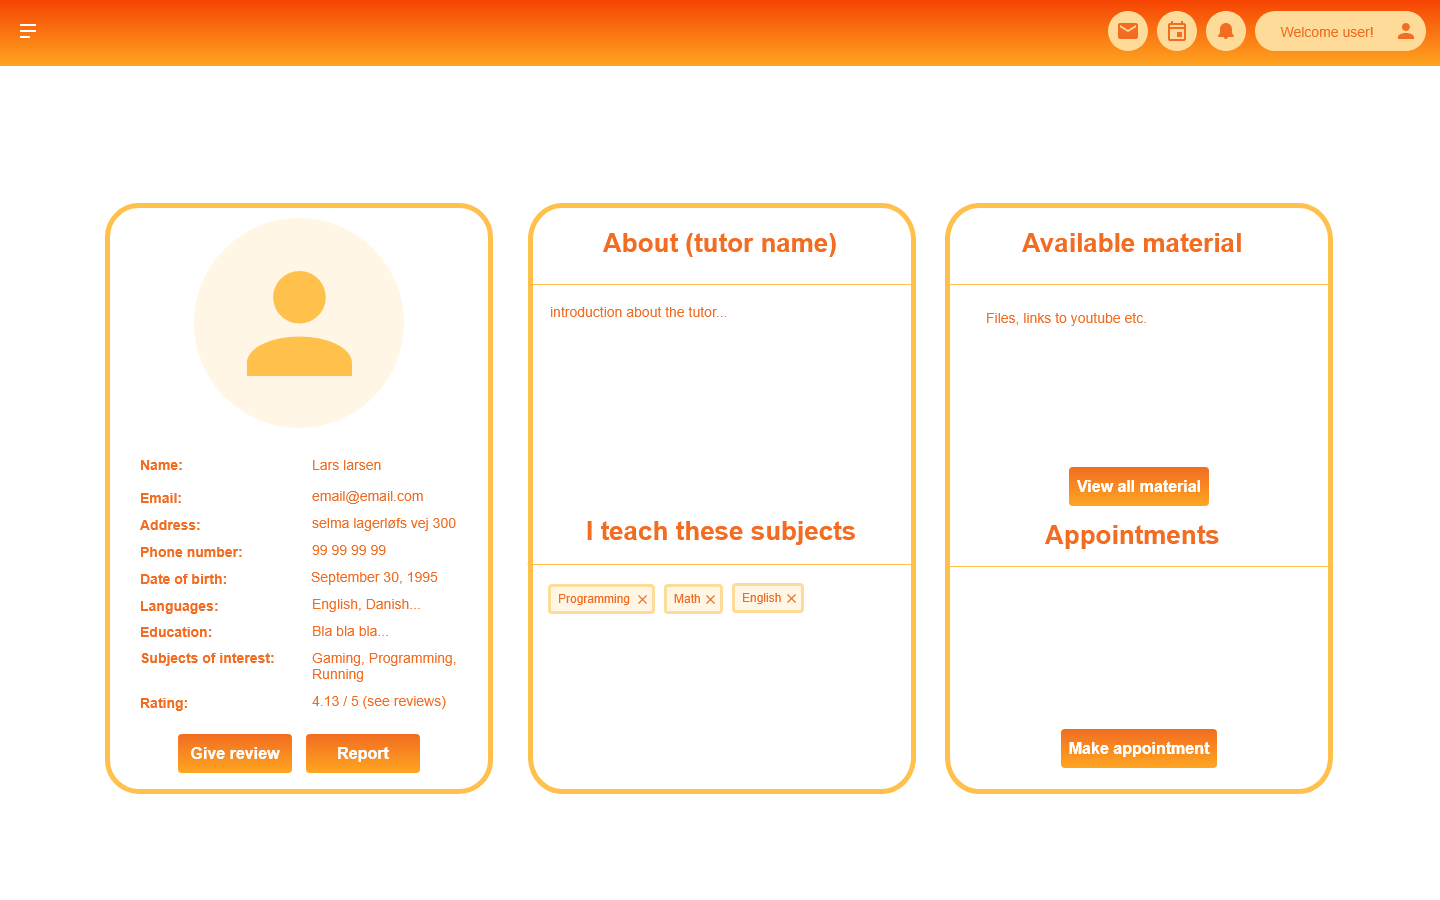
\includegraphics[width=\linewidth]{/prototypes/view-information-on-tutor.png}
     \caption{The page where other users can view information about a specific tutor}
     \label{fig:view-information-on-tutor}
 \end{figure}
This is the page where other users can go and view information about another tutor. 
Much information should be available here so that a user can know if this tutor can be helpful to them.
The page will show basic information on the left side and also show the tutor's rating. 
A user can click \textit{see reviews} to see what other users wrote about the tutor. 
The user viewing the tutor's page can also leave a review of the tutor or report the tutor if they had a bad experience. 
The tutor can display some written information about them in the middle that others can read. 
The middle also shows which subjects the tutor teaches. 
A tutor also has some material connected to their page if they have uploaded any. 
They can make this available to others however they wish, but can also lock it behind payment or only make it available if a student books an appointment with the tutor.
Users can click the \textit{View all material} button to go to the view material page where all the files and links can be found. 
Finally, the user can wish to make an appointment with the tutor. 
By clicking the \textit{Make appointment} button, the user is redirected to the tutor's calendar, where they can find a suitable date for the appointment. 


 \begin{figure}[H]
    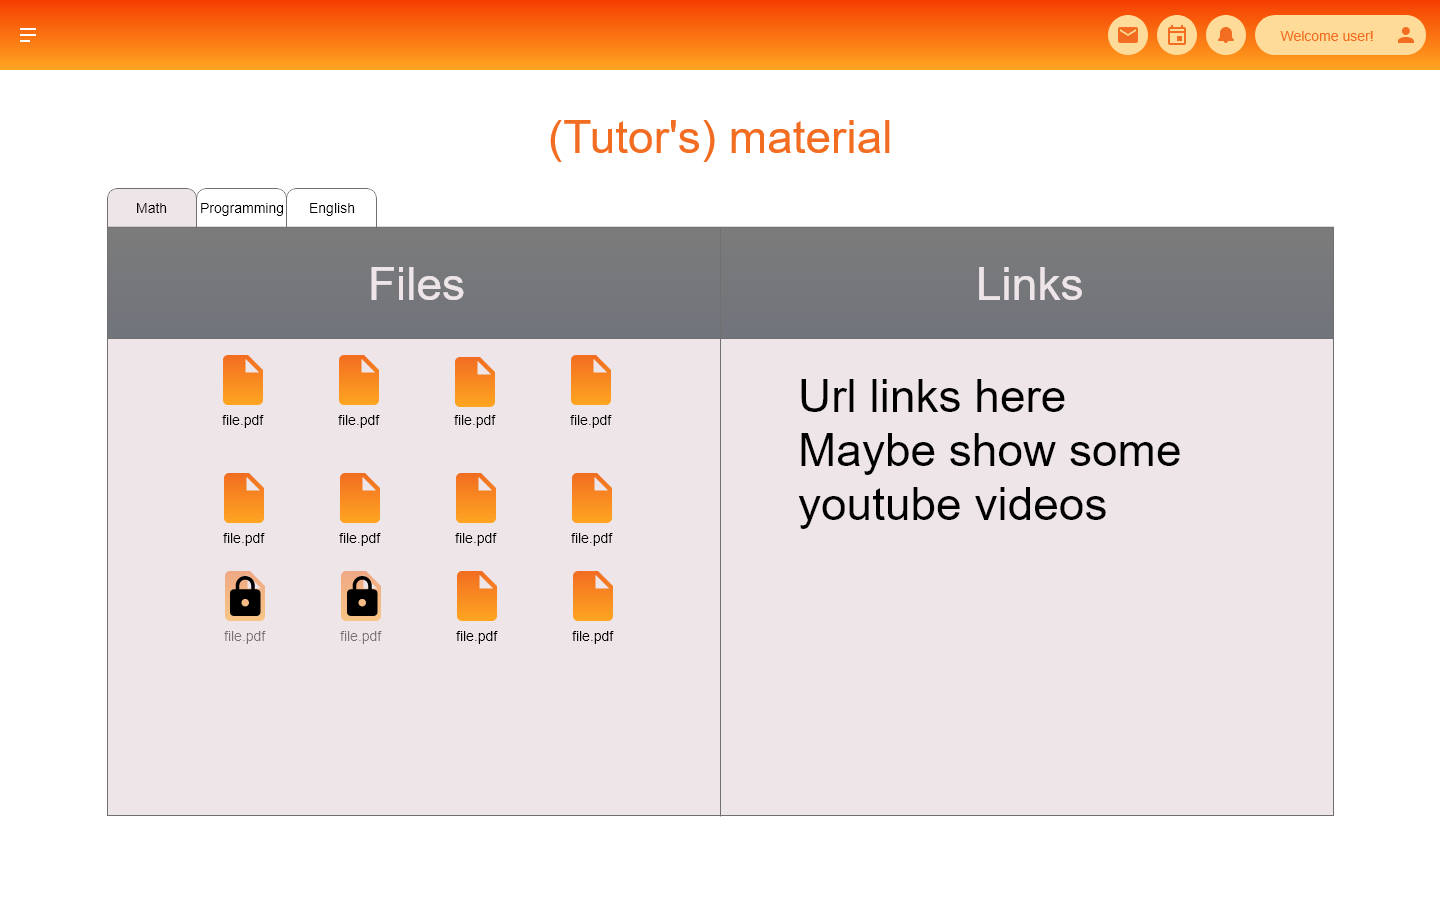
\includegraphics[width=\linewidth]{/prototypes/view-tutor-material.png}
     \caption{The page that shows a tutors available material}
     \label{fig:view-tutor-material}
 \end{figure}
This page shows a specific tutors uploaded material. 
The material is divided into which subject it belongs to make it easier for other users to find the relevant material. 
The material can be any kind of file, or it can be links to useful pages such as some reading material or perhaps a YouTube video. 
When a specific user goes to a tutor's material page, only the material that is accessible to them should be made available. 
All other files should show a lock on top of the file or link to indicate that this item is not available. 
The user can then hover over this item, and it should then tell the user how it can be unlocked. 

\section{Class diagram}
A class diagram helps to create an understanding of the design of the system.
\begin{figure}[]
    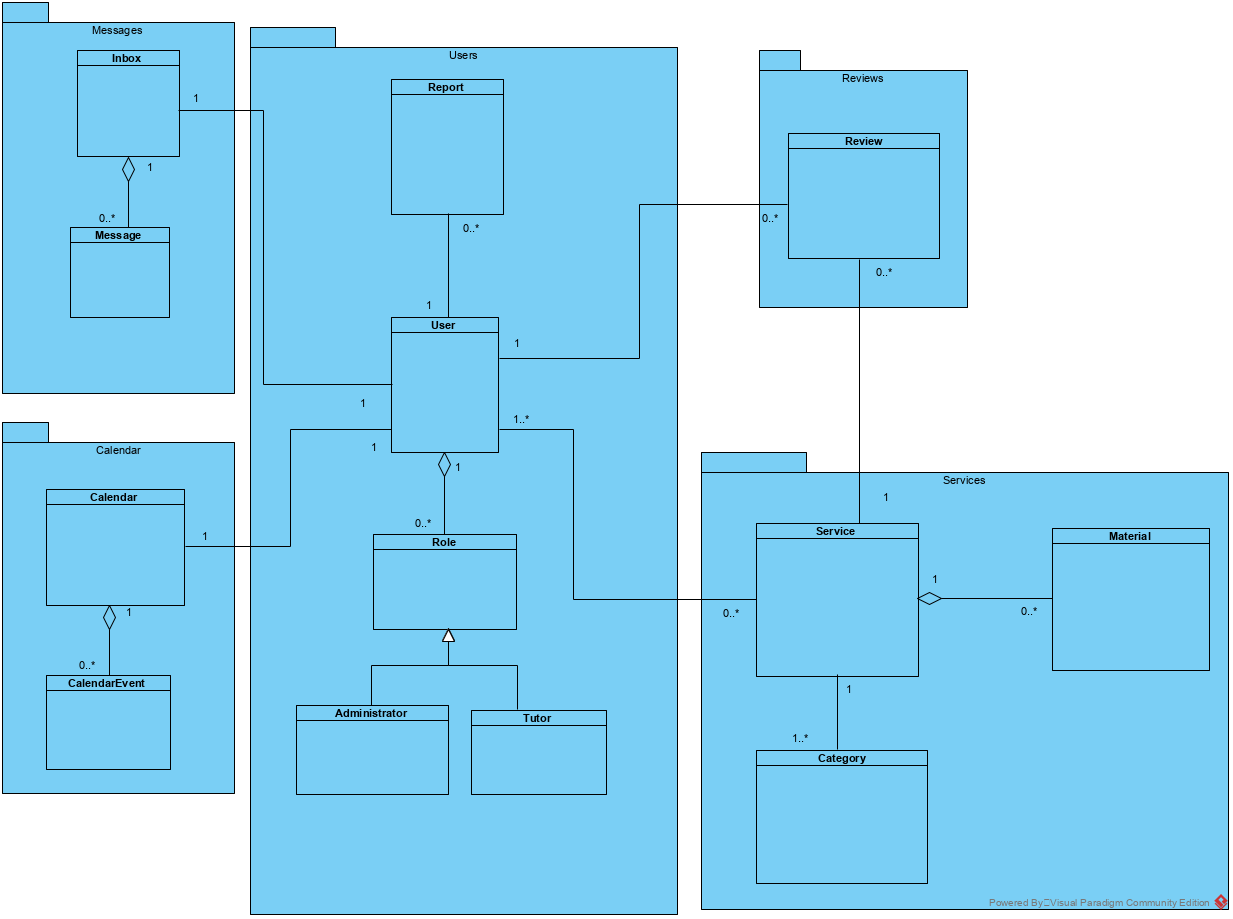
\includegraphics[scale=0.55]{/tutorclassdiagram.png}
     \caption{The class diagram describing classes in the problem domain}
     \label{fig:class-diagram}
 \end{figure}
The diagram in \autoref{fig:class-diagram} illustrates the relevant classes related to the problem domain for the system.
It illustrates structural relations between classes and objects\cite{OOAD}.

\subsubsection{Users}
Users are defined through the \texttt{users} cluster.
A user aggregates 0 or more roles, which is a generalization of either the tutor or administrator classes.
The role class ensures that the user can have both of the different roles, only one role or neither role, and that it can be dynamically changed.
If a user does not have a role, the user is simply regarded as a user of the system - a person seeking a tutor.
Reports are used to ensure that the system is trustworthy and prevent the same problems recurring in interactions between students and tutors.
A user is associated with reports through an association relation.
They will be associated with 0 or more reports, depending on how many times the student has reported reported a tutor.
A report is associated with exactly 2 users, one being the student creating the report, and the other being the tutor to which the report is targeted.
Users are associated with 0 or more reviews in the same way, as students can rate their interactions with a tutor through a review.
If a review is created, it is associated with exactly 2 users as well, since both the tutor being reviewed and the student doing the review are necessary.

\subsubsection{Calendar}
The calendar is the part of the system through which students and tutors establish dates on which to meet.
One calendar is associated with one user.
A calendar aggregates 0 or more calendar events.
The calendar does not need an event, it can simply show the overall view of the month without any scheduled appointments.

\subsubsection{Messages}
Users can send messages through the system.
To facilitate this, users are associated with an inbox.
This inbox aggregates 0 or more of the user's messages.

\subsubsection{Reviews}
Reviews are made by students and are used to review the services of a tutor.
Since users make the reviews, they are associated with 0 or more reviews.
The user could have reviewed multiple services, or none at all.
The reviews are made for a particular service, meaning a service will be associated with 0 or more reviews, depending on whether or not any students have left any reviews for the service in question.

\subsubsection{Services}
A service is what the tutors provide through the system.
A user is associated with a service.
The user can be associated with 0 or more services, meaning that if the user is not a tutor they do not need to provide a service, and if they are a tutor they can provide more than one. 
In the same way, if the user is a student, they do not have to be associated with a service.
The service itself is associated with one or more users.
If the service exists, it may not necessarily be associated with any students, but it is always attributed to at least one tutor.
If the service only consists of material and is based around self studies, it could have multiple tutors authoring it, meaning it would be necessary to attribute the service to both.
A service aggregates 0 or more materials.
The tutor can choose to provide material for their service, as long as it is relevant.
However, a service could also simply be the tutor teaching the student in person, without material provided through the system.
Categories define the subject matter of a service, meaning a service is associated with one or more categories.
If a service is provided, it is based around a subject that defines its category.
However, the service might be related to more than just that one category.
The category assigned could be more specific to provide more information for the student, such as trigonometry rather than mathematics.
In such cases it would likely also be valuable to be able to assign multiple categories.
A category should also be able to exist without being associated to a service, meaning its multiplicity should be 0 to many.
\section{Component architecture}
A component architecture diagram is useful to illustrate how a system is connected.
A component architecture is a system structure composed of interconnected components, where components are a collection of program parts that constitute a whole \cite{OOAD}.
\autoref{fig:architecture-diagram} shows the component architecture.

\begin{figure}[]
    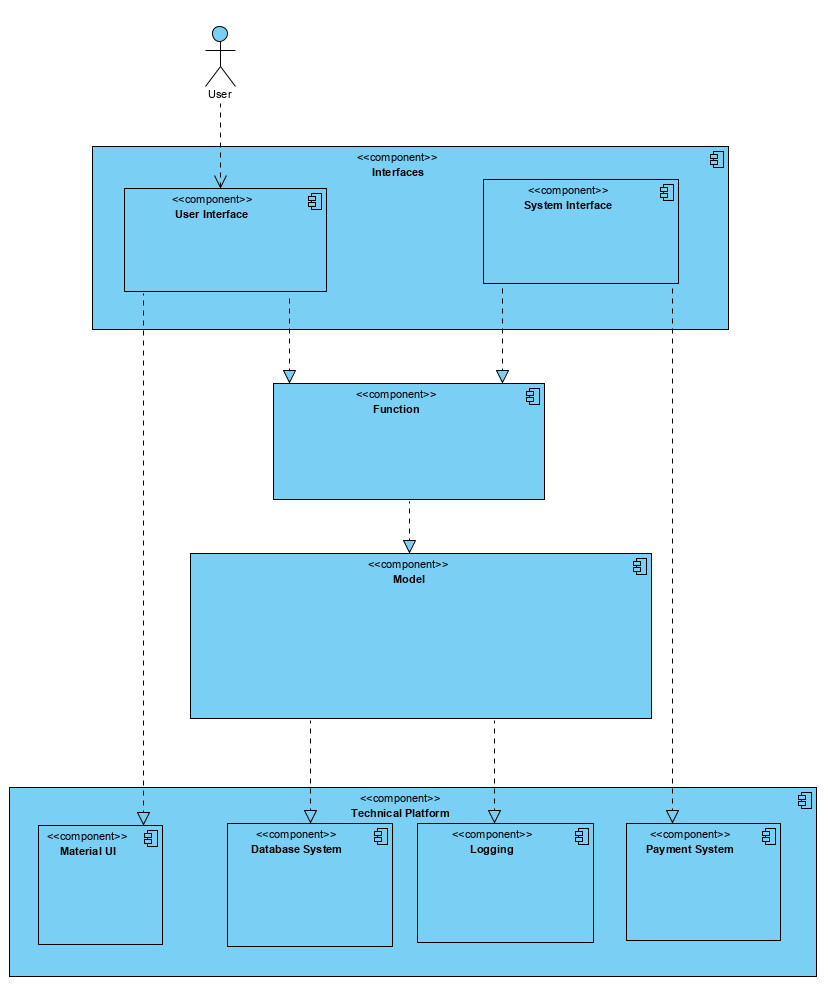
\includegraphics[width=\linewidth]{/architecture.PNG}
    \caption{The component architecture of the system}
    \label{fig:architecture-diagram}
\end{figure}

\subsection{Interfaces}
The top component layer of the system is the \textit{Interfaces} layer.
This layer defines the components that interact with other entities, such as users or other systems, which is how the layer is split.
The user of the system interacts with the user interface.
The user interface has an interface to the \textit{Technical Platform} component layer, more specifically the \textit{Material UI} component.
Material UI is the framework used to create the user interface, which is why they interface.
The user interface also interfaces with the \textit{Function} component, in order to facilitate interaction with the system when used by a user. 
The \textit{System Interface} component interfaces with the \textit{Payment System} from the \textit{Technical Platform}, since a payment system should be used to facilitate transactions.
It also interfaces with the \textit{Function} component, to facilitate interaction with the system.

\subsection{Function and Model components}
The \textit{Function} and \textit{Model} components define the core functionalities of the system.
The function component takes the necessary information from the system and user interfaces, and ensures it can be used by the model.
For example, a user inputs certain information when registering. 
The function component then takes this information, ensures it has the proper format and passes it to the model component.
The model component takes information from the function component, and interfaces with the \textit{Technical Platform}.
From the \textit{Technical Platform} layer it interfaces with the \textit{Database System} and the \textit{Logging} component.
The model's content is received and stored in the \textit{Database System}.
Whenever certain actions are performed through user actions, the \textit{Logging} component takes the relevant model content and logs it.
\\\\
Now that the architecture has been defined and prototypes created, we will discuss how, and with which frameworks we will be creating the front end.


\section{Single Page Application or Multi Page Application}
There are two types of applications that can be created.
One is a \textit{Single Page Application} (SPA), the other is a \textit{Multi Page application} (MPA).
In this section we will be looking into the two types of architectures and explore the advantages and disadvantages that they have.

\subsection{SPAs}
What an SPA allows you to do is build an application that simulates that of a desktop application. 
When a new page is loaded only the necessary content of the previous page is updated.
JavaScript is often used when developing SPAs but it is often used with some library or framework like React to make the development easier.
There are also other frameworks such as Angular or Vue which allow for development of dynamic web applications just as React does. 
\\\\
The main advantage of an SPA is the high speed that comes with the unnecessity of having to load all elements with each new page.
You only need to load the changed elements. 
The frameworks used also make fast development possible because of the powerful tools that are provided. 
It is also easy to create a mobile app based on the finished code of an SPA \cite{SPAvsMPAMerehead}.
SPAs also have great caching possibilities and the local data can be used offline when the user has problems with their connection. 
The pages can then still be shown to the user even with connectivity issues and the local data will be synchronized once the connection is established again \cite{SPAvsMPARuby}.
\\\\
A disadvantage of an SPA is the poor optimization for search engines.
Most of the pages will not be available to scan because of the way an SPA works. 
Some users will also have JavaScript disabled in their browsers, and since the SPA is reliant on JavaScript to load new page content all the time, the pages will not be able to load correctly.
Generally SPAs have less security but with use of the modern frameworks mentioned the security of the page is significantly improved.
SPAs also can not take advantage of browser history since the back button will not go to the previous page since there is only one page. 
There are, however, solutions that can be used for this issue such as using a history API \cite{SPAvsMPAMerehead}.

\subsection{MPAs}
MPAs are different to SPAs in that they have a more standard architecture.
When a new page is loaded it will send a request to the server and all the data will be updated even if it is just a small amount.
A MPA will therefore spend a bit more time loading a new page because it has to update everything.
Actions can be taken to increase the loading speed, however. 
Libraries such as jQuery can be used.
Another popular thing to do to reduce load times is use filters for searching through a list of items as filters do not require a reload of the page.
MPAs are generally used for web applications with a number of pages that have static information such as text, images and links to other pages.
The content of an MPA will be split into many pages with many links to other pages to allow for greater performance.
\\\\
Advantages of MPAs are their ability to optimize their pages for search engines which will make them more accessible to others. 
They are also easy to develop on since the larger technologies, such as the frameworks mentioned for SPAs, are typically not needed \cite{SPAvsMPAMerehead}.
MPAs have unlimited scalability since new content can be placed on new pages with no limitations whereas SPAs are more limited by the amount of content that can be placed on a single page without having it affect performance \cite{SPAvsMPARuby}.
\\\\
Disadvantages of MPAs are the slower performance that comes with having to load all the content every time a page is loaded.
It will generally also take more time to develop an MPA since it is difficult to separate the frontend and backend as they are closely knit together.
Maintenance of an MPA can also take significantly longer than for an SPA since it will only take more time to update every time a new page is added \cite{SPAvsMPARuby}. 

\subsection{Why SPA}
For this project we have chosen to build the frontend of the system using the React framework. 
With React it is most common to build SPAs, but it is also possible to build MPAs. 
For this project we will be building an SPA.
The system will not have that many pages with a lot of static information so this is not a needed feature for the system.
We want the UI of the system to be very responsive to the user's input and also have a great response time when updating elements of the page which is inline with the choice of an SPA.
The possibility to cache data and then making use of that for cases where a user has a poor connection is also inline with some of the things discussed in \autoref{sec:scalability}.
We also do not need our system to be optimized for search engines since most parts of the system will only be available to users that are logged in.
Accessibility of the system from mobile devices is also desired and with an SPA it is much easier to make this available. 
Because of these points an SPA will be a great fit to the type of system that we are building.

\section{Why React}
For our front end, we decided to use React.
React is a JavaScript library for creating web applications \cite{ReactJS}. 
\\
React is one of the most popular choices when it comes to front end development \cite{NPMVueReactAngular}.
It is created by Facebook and used for their website as well as numerous other websites \cite{ReactHistory}.
React is lightweight and allows the user to choose what additional libraries they would want to use in their project, which keeps the size of the project down.
\\
It also has an extensive ecosystem that offers various react specific libraries that one could use in their web applications.
Being this popular results in a very robust ecosystem with lots of users, but this is also needed as the additional libraries are maintained exclusively by the react community and are not a part of the core React library, unlike other front end libraries such as Vue \cite{Vue}.
\\
React was created so that it would be easier to make reusable UI components that can handle data that changes regularly \cite{ReactHistory}.

\todo{Cites her er fucked?}
\section{Introduction to React}\label{sec:intro-to-react}
In this section we will look at the different building blocks and concepts of React.
React will often be used with a syntax extension to JavaScript called JSX \cite{introducingJSX} which makes it possible to declare variables that resemble HTML code.

\begin{center}
    \texttt{const element = <h1>Hello, world!</h1>;}
\end{center}
This variable declaration can be called a React element which can then be rendered to the Document Object Model (DOM) of the web page.
With React, it is possible to render the element to the DOM by using \texttt{ReactDom.render()}.
The element is passed to this function as well as the DOM node we would like it to be rendered to.
In this case we are rendering the React element \texttt{element} to the DOM node \texttt{root}.

\begin{center}
    \texttt{ReactDOM.render(element, document.getElementById('root'));}
\end{center}
A nice feature of JSX is that it allows you to include dynamic content in HTML, by including JavaScript variables wrapped in curly braces to indicate that they should be evaluated by the JavaScript engine upon rendering.

\begin{lstlisting}
const name = 'Josh Perez';
const element = <h1>Hello, {name}</h1>;

ReactDOM.render(
  element,
  document.getElementById('root')
);
\end{lstlisting}
The variable that is embedded in the JSX can be any valid JavaScript expression \cite{introducingJSX}.

\subsection*{components}
In React components are used, which are files that hold all of the logic, HTML and styling that is needed.

\begin{lstlisting}
import React from "react";

function App() {
    return (
        <div>
            <h1>Hello React</h1>
        </div>
    );
}

export default App
\end{lstlisting}
In this example we create the component \texttt{App} and export it.
By exporting it we can use the \texttt{App} component elsewhere and render it.
In the function we return a JSX element which React will then compile to regular JavaScript that can be understood by the browser.
The idea is to build the UI from components by exporting them and then importing them into other larger components to contain them.
This means that the components act as the building blocks of the UI because they can be reused in other components.
\begin{lstlisting}
import React from 'react';

function Button() {
    return (
        <div>
            <button onClick={console.log('Hello')}>Hello React</button>
        </div>
    );
}

export default Button
\end{lstlisting}
As an example we can create a button component with an on-click event embedded into it.
Here we use brackets to enable us to embed a callback function in the JSX which will be called when the button is clicked.
We can now export this button and it can be imported by other components.
There are both class components and functional components.
An example of this can be seen in \autoref{lst:on-click-example-1} and \autoref{lst:on-click-example-2}

\begin{lstlisting}[caption={Example of a button with a onClick event in a functional component},label={lst:on-click-example-1}]
function Button(props) {
	return (
		<div>
			<button onClick={console.log(props.textToPrint)}>Hello React</button>
		</div>
	);
}
\end{lstlisting}

We can convert this into a class like this:

\begin{lstlisting}[caption={Example of a button with a onClick event in a class component},label={lst:on-click-example-2}]
class Button extends React.Component {
	constructor(props){
		super(props);
	}

	render() {
		return (
			<div>
				<button onClick={console.log('Hello')}>Hello React</button>
			</div>
		);
	}
}
\end{lstlisting}

A component is conceptually a JavaScript function or class, which means that they can accept inputs called \texttt{props} which can contain data that can be used in the React elements.
If a component is used in another component, we can use \texttt{props} to pass data to the child component.
\subsection*{Props}
When a component is instantiated it is possible to pass an arbitrary number of arguments to the component by passing key and value pairs.
These are then accessed through the props object in the component.
An example of this can be seen in \autoref{lst:react-props-lsting}.

\begin{lstlisting}[caption={An example of how properties are passed to children components}, label={lst:react-props-lsting}]
function Site(){
	const titleVariable = 'title';
	const descriptionVariable = 'This is a component';

	return <TextComponent title={titleVariable} description={descriptionVariable} />;
}

function TextComponent (props){
	return (
		<div>
			<h1>{props.title}</h1>
			<p>{props.description}</p>
		</div>
	);
}
\end{lstlisting}

The props of a component should be treated as read-only because any changes to the props will not be reflected in the rendering of the component.

\subsection*{State}
There two kinds of components, which are stateful and stateless components.
In our application we will mostly implement stateful components as class components and stateless components as functional components. 
Functional components can also be stateful, but the choice of using class components is mostly a question of preference.
A stateful component has a state which contains all the dynamic data in the component.
This is useful since the render method is called every time the local \textit{State} is changed.
We can set the initial state of a component by assigning \texttt{this.state} in the constructor of the component.
\begin{center}
    \texttt{this.state = \{textToDisplay: 'Initial text'\};}
\end{center}
The state can then be changed by reassigning to the \texttt{date} variable.
This is done by using the \texttt{this.setState()} function.
\begin{center}
    \texttt{this.setState(\{textToDisplay: 'New text'\});}
\end{center}
Parent or child components should not care if a certain component is stateful or stateless since the state is local and not accessible by other components.
A component can however pass variables from its state through \texttt{props} to a child component, which means that information about a state can only be passed in a \textit{top-down} approach \cite{ReactJS}.
Every time a state is changed with \texttt{this.setState()} the component that the state belongs to and all of its children are re-rendered.
By passing callback to the props of children we can allow  the children of a component to transfer data back to its parent and even trigger re-renders by passing callback functions that set the state of the parent component.
If a function calls \texttt{this.setState()}, it has to be bound in the constructor of the component.
An example of how this is done can be seen in \autoref{callback-example}.
\begin{lstlisting}[caption={An example of a callback function}, label={callback-example}]
class ourComponent extends Component {
	constructor(props){
		super(props);
		this.state = {
			textToDisplay: 'initial text'
		};

		this.handleChange = this.handleChange.bind(this);
	}

	handleChange(text){
		this.setState({
			textToDisplay: text
		});
	}

	render(){
		return <ChildComponent handleChange={this.handleChange} />
	}
}
\end{lstlisting}

\subsection*{Lifecycle}
When a component is implemented as a class that extends \texttt{Component} from the React library, it gives us access to some functions that are automatically called at different points in the lifecycle of a component.
The function that we will mostly be using is \texttt{componentDidMount}.
This function is called right after the component is rendered for the first time in its lifecycle.
This is useful for when we need to fetch data from the API that we want to save in the state of the component.
The reason that this is not done in the constructor of the component is that the render function should not be waiting for asynchronous operations before it is allowed to render.
This is because we do not know how long it will take before the asynchronous function is done executing, or if it will even succeed.
Instead of waiting, it is better to first render the component before calling asynchronous functions that will trigger a re-rendering of the component.
\begin{lstlisting}[caption={Example with the componentDidMount function}, label={lst:componentDidMount-example}]
class OurComponent extends Component {
	constructor(props){
		super(props);
		this.state = {
			data: null
		};
	}

	componentDidMount(){
		userService.getUserById(1).then((dataRes) => {
			this.setState({
				data: dataRes
			});
		})
	}

	render(){
		if(this.state.data !== null){
			return <ChildComponent data={this.state.data} />:
		}
			
		return null;
	}
}
\end{lstlisting}
An example of \texttt{componentDidMount} can be seen on \autoref{lst:componentDidMount-example}.
We initialize the state with a null.
We check in the render function if the value in the state is null.
If it is null we return null, which just renders nothing.
If it is not null we render a component and pass the data as a prop.
The first time the render function is called, the value is null.
After it has rendered the \texttt{componentDidMount} function is called.
In \texttt{componentDidMount} we make an API call and then set \texttt{data} in the \texttt{state} equals to the response.
Because the state is changed the \texttt{component} re-renders and \texttt{ChildComponent} is rendered this time.
\\\\
Finally we will take a look at designing an API, and choosing and designing a database.

\section{API design}
When designing an application with scalability in mind, the API must be able to handle both a small and large amount of requests and give a response that can be used across platforms, in case the system needs to be scaled to other platforms such as a desktop application or a mobile application.\\
Before going into the specifics of how the API should be designed, let us have a closer look at how APIs work.

% Define block styles
\tikzstyle{block} = [rectangle, draw, fill=blue!20,
    text width=5em, text centered, rounded corners, minimum height=4em]
\tikzstyle{line} = [draw, -latex']

\begin{figure}
\centering
\begin{tikzpicture}[node distance = 3cm, auto]
    % Place nodes
    \node [block] (appcli) {Application / client};
    \node [block, right of=appcli] (request) {API requests};
    \node [block, below of=request] (serverdata) {Server / data source};
    \node [block, left of=serverdata] (response) {API response};
    % Draw edges
    \path [line] (appcli) -- (request);
    \path [line] (request) -- (serverdata);
    \path [line] (serverdata) -- (response);
    \path [line] (response) -- (appcli);
\end{tikzpicture}
\caption{Workflow of an API} \label{fig:api-workflow}
\end{figure}

The flow of using the API starts with the application or client, which will be responsible for sending a request to the API for the information it needs to finish its computations.
This request will inform the API about what data it needs in the request.
To simplify this, we present an example:\\
The client wants to render a page with information about a course; to do this, it would need all data associated with this course.\\
This information will generally be exchanged by sending a request to the API that could look something like \texttt{api/course/2}, where 2 is the unique ID of the course.
\\
The API will now be responsible for fetching this information from the database layer or another data source. 
Once that has been completed, the response will be returned to the client so it can finish rendering the page with the newly received data.
\\
This process is illustrated on~\autoref{fig:api-workflow}.

\subsection{Language}
One of the first decisions that must be made when developing the API is which programming language to use.\\
For this project, it was decided to use the React JavaScript library for the frontend design.
To keep the codebase as consistent as possible in terms of code structure, it was deemed suitable to use the same language for the API.\\
In addition to keeping the codebase uniform, Node.js offers an extensive package manager, which allows for easy inclusion of existing Node.js modules by other developers.
One of those modules is \texttt{Express}, which is a web application framework for Node.js, that includes a series of utilities related to creating web applications and APIs.

\section{Database choice}
The system being developed during this project is heavily focused on scalability, it is therefore important that a database system that can handle a lot of data and which makes scalability easier is chosen.
\\
Furthermore our application is going to handle a variety of data forms. It will store both structured data in the form of user profiles as well as unstructured data such as pictures and videos.
\\
This means that both a relational and non-relational database system could work, making the choice more difficult.
We considered going with a non-relational database, as such database system is often used with our frontend framework React, but since the team has more experience working with relational databases it was decided to go with this kind of database system.
\\
The following databases were looked incorporates
\begin{itemize}
    \item Postgres
    \item MySQL
    \item Oracle
    \item MariaDB
    \item Microsoft SQL Server
\end{itemize}
Postgres is the most advanced opensource relational database \cite{Postgres}.
It is free and is one of the most popular databases being used\cite{databasePopularity}.
It has great documentation and a large active user base.
Furthermore it is not only a relational database but a object-relational database which gives it support for user-defined objects, functions, operators and more.
It also allows storing of Json objects and can therefore be used almost akin to a non-relational database.
Postgres is also ACID compliant, meaning that a database transaction is ensured to be completed even in the event of errors or even power failures.
\\
\\
MySQL is the most popular database used today\cite{databasePopularity}.
It is almost completely open source and has a very active community\cite{MySQL}.
MySQL has also added the functionality to act akin to a non-relational database.
MySQL is not ACID compliant.
\\
\\
Oracle is a commercial database and is quite expensive to obtain\cite{oracle}.
Furthermore you have to pay for extra features.
For these reasons it was decided against using this database.
\\
\\
MariaDB is also a opensource relational-database\cite{MariaDB}.
Just like Postgres it is ACID compliant, can store Json objects and has good documentation.
\\
\\
Microsoft SQL Server is a commercial database system\cite{MSSQLSERVER}.
Like Oracle it means to have access to the full system.
\\
\\
It was decided to use Postgres as the database system.
This was because Postgres also incorporates the ability to handle unstructured data in much the same way a non-relational databases does it, giving us the means to explore that aspect of database design if needed.
The ACID compliance was also deemed important which removed MySQL from the selection process. 
The group also has some experience working with Postgres from an earlier database course which was the last reason to pick it over MariaDB.

\section{Entity-relationship diagram}
An entity-relationship diagram (ER diagram) can express the structure of a database graphically\cite{DBConcepts}.
This is a way to gain a better understanding of the requirements of the database and to ensure its design is clear.
An ER diagram shows entity sets of the database and their relationships.
An entity is a thing or an object in the real world that is distinguishable from other objects, and are described through a set of attributes.
An entity set is a set of these entities.
Relationships are associations between entities.
Cardinalities are important for these relationships - they express the number of entities to which another entity can be associated\cite{DBConcepts}, either one or many.
With these two cardinalities, the following mappings can be used:
\begin{itemize}
    \item One-to-one
    \item One-to-many
    \item Many-to-many
\end{itemize}
A one-to-one relationship means that an entity in an entity set A is associated with at most one entity in an entity set B, and an entity in B is associated with at most one entity in A.
A one-to-many relationship means that an entity in A is associated with any number of entities in B, and an entity in B can be associated with at most one entity in A.
For many-to-many relationships, an entity in A is associated with any number of entities in B, and an entity in B is associated with any number of entities in A\cite{DBConcepts}.
The following figure illustrates the physical design of the database for this system:

\begin{figure}[H]
    \includegraphics[width=\linewidth]{}
     \caption{The ER diagram that illustrates the design of the database.}
     \label{fig:er-diagram}
 \end{figure}

In \autoref{fig:er-diagram}, entities are represented by the rectangular boxes.
The name of the entity set is in the header of the box, and the list of attributes is below the name, along with the type of each particular attribute.
\textit{User} is an example of an entity set.
Each entity is defined through the list of attributes shown below the name, such as \textit{ID}, \textit{Username} and \textit{FirstName}.
Relationships are represented by the lines between entities.
The way the line representing the relationship connects to the entity shows the cardinality of that relationship.
If the line ending is connected to the entity by the circle triangle combination, such as both connections to review, it means this side of the relationship has a cardinality of many.
If the line simply ends with another line crossing it such as the ones connected to tutor or admin, it has the cardinality of one.
\\\\
Starting from the left are the \textit{material} and \textit{service} entity sets connected through a relation. 
A material entity has a number of attributes, such as a description of the material, a type such as article, text or video, and a unique identifier known as the primary key.
This primary key is the attribute \textit{ID}.
When an attribute is unique, it can be used to identify a given instance of the entity. 
However, because of the one-to-many relationship between service and material, material also contains what is known as a foreign key in the attribute \textit{ServiceID}.
This foreign key references the primary key of the entity set that participates as the one side. 
This ensures that for any entity in set \textit{material} you can use the foreign key to get the corresponding service.
\\\\
The relationship between \textit{service} and \textit{category} is a many-to-many relationship.
To model this, a separate entity set is created.
This entity set is named after the two participating sets, and has both primary keys as its attributes.
This ensures that for a particular entity in the set \textit{service}, it can be related to multiple entities of the set \textit{category}.
In the database, this would be achieved through multiple entities of the \textit{service_category} being present with the same \textit{ServiceID} attributes, but each instance is linked to a different \textit{CategoryID} attribute.
Another example of a many-to-many relation is users and messages.
A message is associated with a sender, and at least one receiver.
\\\\
A particularly interesting entity set is the \textit{user} set. 
As defined in the \autoref{REF TIL CLASS DIAGRAM}, the admin and tutor properties are viewed as specializations through roles.
This is achieved in the ER diagram by modelling them as subtypes, defining an \textit{ISA} relationship.
This is what the arrow from both \textit{tutor} and \textit{admin} represent.
They show that a tutor is a user, and in the same way, an admin is a user.
The user entity set also has multiple connections to certain other entity sets - \textit{service} and \textit{report}.
The reason for this is due to the subtypes. 
As a user can be both a student and a tutor, this needs to be reflected in the relationships.
Many users can be associated to a service - the only limit is how many students a tutor can have at a time.
A service is however associated with one tutor.
As such we chose to model it through two relationships - one that is one-to-many for the tutor as a tutor can have multiple services, but each service is associated with one tutor, and a many-to-many for students.
A report is made by a student targeting a tutor. 
as such, we model it through two relations to the user entity set, in order to get a foreign key for both the reporting student and the tutor being reported.



\section{Recommender system}\label{Recommender-system}
It would be beneficial to provide a way for users to see relevant, interesting services for their preferences, in order to make the system more usable.
For example, given the personas defined in \autoref{sec:personas}, it would be beneficial for Storm or Peter to have some recommendations for what they should try out.
To accomplish this, a recommender system can be used.
The following section will detail different ways of implementing such a system and which one we chose to implement.

\subsection{The purpose of a recommender system}
When searching for something new, information overload can occur.
Many different sources can provide information that might not be relevant.
If a new user interacts with this system, seeking to find a new subject in which to attain knowledge, this user could potentially be presented with an overwhelming amount of services, depending on how many tutors have made these available.
Another issue that might arise is that not all of the services will be relevant for the new user, serving only to clog the list of services. 
This leads to information overload, where the retrieved information in the form of services is not what the user needs, and not enough of the correctly relevant information is returned.
Recommender systems are used to remedy these issues.
They help match users with relevant items, in this case services, to ease the information overload.
This generates value for both the user and the tutor, in that users are matched with what they have a predilection for, and tutors can reach more prospective students.
We discuss two methods of creating a recommender, \textit{content-based filtering} and \textit{collaborative filtering}.

\subsection{Content-based filtering}\label{content-based-filtering}
Content-based recommender systems recommend an item to a user based upon a description of the item and a profile of the user's interests \cite{ContentBasedFiltering}.
A common scenario for web applications is that they present a list of items to a user, and the user then selects among these to receive more details. 
An item in such a scenario would have a representation dependent on the implementation, which could be used to analyze items of particular interest for a user.
Items are often stored in databases, creating structured data with each entry having the same set of attributes. 
This lends itself well to learning a user profile through different machine learning algorithms.
Examples of a basic representation of items and users are shown in Tables \ref{tbl:content-item} and \ref{tbl:content-user}.
As shown, users and items are represented by the same set of attributes.
\begin{table}[H]
    \centering
    \begin{tabular}{|l|l|l|l|l|}
    \hline
    Title                                         & Genre    & Author        & Price & Type      \\ \hline
    Blue Moon                                     & Thriller & Lee Child     & 10    & Hardcover \\ \hline
    Norse Mythology                               & Fantasy  & Neil Gaiman   & 6     & Paperback \\ \hline
    Normandy ‘44                                  & History  & James Holland & 14    & Hardcover \\ \hline
    \end{tabular}
    \caption{This figure shows a possible representation of a few items for content-based filtering.}
    \label{tbl:content-item}
\end{table}
\begin{table}[H]
    \centering
    \begin{tabular}{|l|l|l|l|l|}
    \hline
    Title                                         & Genre    & Author        & Price & Type      \\ \hline
    ... & Fantasy  & George R. R. Martin, J.K. Rowling & 5    & Paperback \\\hline
    \end{tabular}
    \caption{This figure shows a possible representation of a user.}
    \label{tbl:content-user}
\end{table}
\noindent
The basic idea for content-based filtering is then to compute the similarity of an unseen item with the user profile, and suggest the items with attributes that are most similar to those in the user profile..
Unstructured data, such as text fields with no restriction, create complications when creating a user profile, as relationships between the values on an attribute for different items for a specific user can be found, but an unrestricted text will generally be unique \cite{ContentBasedFiltering}. 
If a user liked different restaurants based on the same cuisine, it could be indicated that this user would be likely to like other restaurants focused in the same cuisine as well, but a text review would not necessarily give this information.
Many domains can be represented by semi-structured data where issues arising from certain types of unstructured data, such as text fields, are converted to a structured representation \cite{ContentBasedFiltering}.
A user profile shows the preferences of the user, and consists mainly of two types of information:
\begin{itemize}
    \item A description of the types of items that interest the user
    \item A history of the user's interactions with the recommender system, such as storing the items that a user has viewed and information related to the interaction, such as if the user purchased the item.
\end{itemize}
Historical data of interactions can be used to filter out already purchased items, display recently visited items or as training data.
Creating a model of a user's preferences is then done through a form of classification learning, in which training data is divided into categories, an example being the binary categories \textit{items the user likes} and \textit{items the user dislikes} \cite{ContentBasedFiltering}.
These algorithms learn a function that models a users interests, and given a new item and the user model, this function predicts whether or not the user is interested in the item through a probability or a numeric value by analyzing the item representation and user profile.
Popular learning approaches for content-based filtering are \textit{naïve Bayes}, \textit{nearest neighbor methods} or \textit{linear classifiers}.

\subsection{Collaborative filtering}
Collaborative filtering differs from content-based filtering in that it focuses on matching users and items through the opinions of other people.
Collaborative filtering is based on word-of-mouth recommendations.
A person might have friends that recommend different things, and will eventually learn which of these friends has tastes that most align with their own, and thus which recommendation to value the most.
Collaborative filtering extends this concept \cite{CollaborativeFiltering}.
Collaborative filtering makes use of ratings.
These could be ratings between 1-5 or 1-10, for example, or simply binary ratings.
A rating is an association of two things, a user and a value.
A matrix of ratings can then be constructed, as shown in \autoref{tbl:collaborative-example}.
The empty entries indicate that the user has not rated the item, and are what the system should be able to predict.
\begin{table}[H]
    \centering
    \begin{tabular}{|l|l|l|l|l|}
    \hline
           & Item1 & Item2 & Item3 & Item4 \\ \hline
    Peter  & 3     &       & 5     &       \\ \hline
    Storm    & 4     & 2     &       & 3     \\ \hline
    Jensine   &       & 5     & 3     & 2     \\ \hline
    Anton & 1     &       & 2     & 4     \\ \hline
    \end{tabular}
    \caption{This figure shows an example of a ratings matrix, with ratings from 1 to 5. An empty entry indicates that the user has not rated the item.}
    \label{tbl:collaborative-example}
\end{table}
\noindent
Domains with certain properties lend themselves to collaborative filtering. 
These are \textit{data distribution}, \textit{underlying meaning} and \textit{data persistence} \cite{CollaborativeFiltering}.
Data distribution encompasses domains in which there are many items, many ratings per item, more users rating than items to be recommended and users rate multiple items.
Underlying meaning encompasses domains in which users can have tastes in common, evaluation of an item cannot be done objectively and items are homogenous.
Data persistence encompasses domains in which items persist and taste persists, meaning the tastes of the users do not change rapidly.
\\\\
Collaborative filtering usually makes use of \texttt{k nearest neighbor} algorithms based on users or items, or latent factor models to create predictions.
The user-based nearest neighbor approach focuses on finding users with similar tastes from which to predict a given user's rating, whereas the item-based approach focuses on finding items similar to a given item, and then taking the user's ratings for those similar items to predict a rating for an unrated item.
The latent factor approach focuses on splitting the rating matrix into separate matrices through matrix factorization to simulate communities, and creating predictions from these.


\subsection{Pros and cons}\label{sec:recommender-pros-and-cons}
Content-based filtering and collaborative filtering use different underlying assumptions \cite{CollaborativeFiltering}.
Content-based filtering assumes that items with similar objective features will be rated similarly, whereas collaborative filtering assumes that people with similar tastes rate things similarly, and that customers who had similar tastes in the past will have similar tastes in the future.
\\\\
The assumption that collaborative filtering employs, that users will have similar taste in the future, is quite strong and cannot be guaranteed, as tastes are likely to change over time.
Content-based filtering can predict relevance for items without ratings by looking at similar items, whereas collaborative filtering requires ratings for an item to create predictions.
This means content-based filtering is especially useful for items that change a lot, but it needs content to analyze.
For domains where content is scarce, such as for a system in which users rate movies since a small amount of users will actually leave a rating, collaborative filtering has an edge since it does not require content.
\\\\
Content-based techniques can have problems with new users, as there is a ramp-up phase when learning a model of the user's interests.
To do so, it needs explicit or implicit feedback, and there is no guarantee that the user leaves explicit feedback such as a rating, and implicit feedback from a user's behavior can be imprecise.
Since collaborative filtering requires ratings for an item to create predictions it has issues with cold starts.
If a new item is added, it will not have any initial ratings from users, which means creating a prediction becomes different as it has nothing from which to base the prediction.
\\\\
Collaborative filtering methods making use of \texttt{k nearest neighbor} methods can have scalability issues, as the rating matrix can grow to be very large as more users join the service or more items are added.
This is a problem that latent factor models alleviate, as they reduce the size of the rating matrix through splits.
Content-based and collaborative filtering are not mutually exclusive, and both can be used in a complementary fashion to avoid some of the issues that arise when using just one.
\begin{table}[]
    \begin{tabular}{|p{.2\textwidth}|p{.4\textwidth}|p{.4\textwidth}|}
    \hline
                    & Content-based                                              & Collaborative                                                             \\ \hline
    Assumptions     & Items with similar features are rated similarly            & People with similar taste rate items similarly, taste will not change     \\ \hline
    Requirements    & Does not need ratings, but content to analyze              & Needs ratings but not content                                             \\ \hline
    Item changes    & Deals well with changing items by looking at similar items & Does not deal well with new items, as it needs initial ratings on an item \\ \hline
    Start-up issues & New users can have large ramp-up                           & Cold starts with new items                                                \\ \hline
    \end{tabular}
    \caption{A comparison of the pros and cons}
    \label{tab:recprosandcons}
    \end{table}

\subsection{Our choice}\label{subsec:recommender-our-choice}
Ideally, a combination of both collaborative and content-based filtering is ideal.
However, for this project implementing such a combination was not feasible, and we had to focus on one type of recommender system.
The reason it was not feasible was due to the recommender system being based on knowledge acquired from one of the semester courses, and such systems were only detailed towards the end of the semester, leading to a lack of time to create a combined solution.
\\\\
The system has a simple rating system in which users rate a service on a numerical scale of one to five.
It is assumed that services will be rated by a small subset of users, since not all users will participate in all services, and not all who participate in a given service will leave a rating of it.
This means the domain will have content that is scarce.
It is also assumed that services will not change a lot.
If a service is based around swimming, we do not expect that it will quickly be changed to feature another subject matter, but rather a new service be added by the same tutor with the new subject matter.
\\\\
As such, the better choice would be collaborative filtering, as the domain lends itself more to this type of system.
In terms of which approach to collaborative filtering to use, the added scalability of a latent factor model provides it an edge for this system as it focuses on scalability.

\subsection{Collaborative filtering through a latent factor model}
The latent factor model approach to collaborative filtering is an approach that tries to explain the ratings by characterizing both items and users on a number of factors.
This number of factors is usually 20-100 \cite{MatrixFactorization}. 
The factors are thought of as measures that measure dimensions.
For example, for movies, the factors could be thought of as measuring obvious dimensions such as amount of action, less well-defined dimensions such as character development or uninterpretable dimensions \cite{MatrixFactorization}.
\autoref{fig:latent-factor} shows an example of a latent factor approach with two dimensions.
It shows an example of how users and movies could be characterized based on the dimensions.
A user's predicted rating for a movie would then be equal to the dot product of the user's and movie's location on the graph, for example, user 5 would be expected to like movie 1, think movie 4 is average and dislike movie 2.
\begin{figure}[H]
    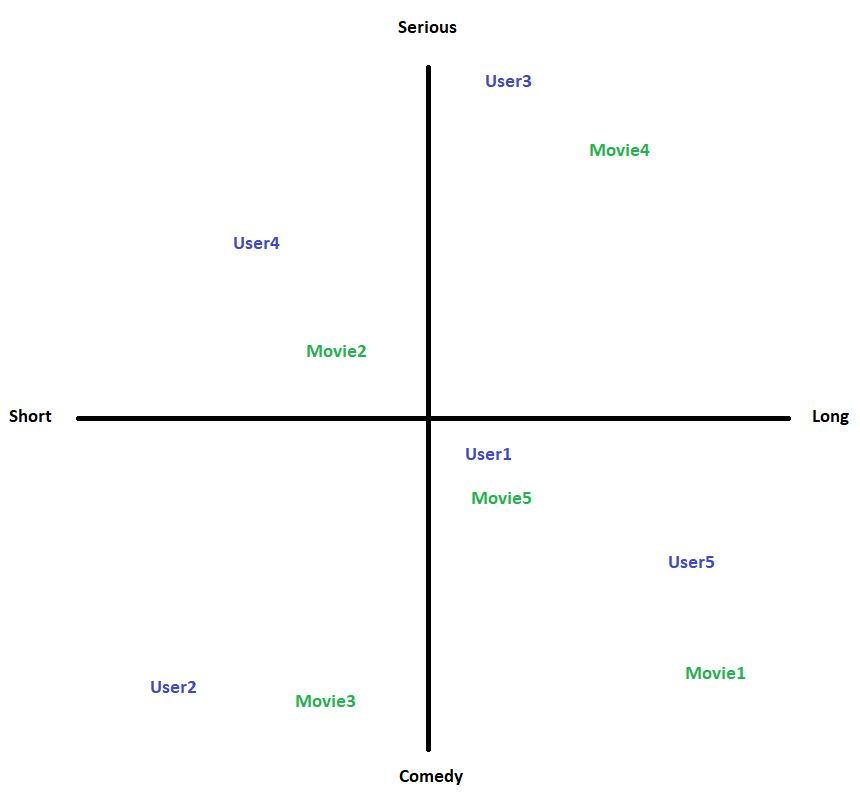
\includegraphics[width=\linewidth]{/recommender/latentfactor.JPG}
     \caption{A simplified illustration of a latent factor approach.}
     \label{fig:latent-factor}
 \end{figure}
 \noindent
A popular method of approaching a latent factor model is through matrix factorization.
Matrix factorization aims to characterize items and users by vectors of factors, and a recommendation would be found by a similarity between these.

\subsubsection{Matrix factorization}
Matrix factorization maps users and items to a latent factor space of dimensionality \textit{f} \cite{MatrixFactorization}. 
This is achieved by taking the ratings matrix and splitting it into two matrices of the following dimensions, where $N_{i}$ is the number of items, $N_{u}$ is the number of users and $f$ is the number of factors:
\begin{equation}
    N_{i} \times f
\end{equation} 
\begin{equation}
    f \times N_{u}
\end{equation}
This results in each item \textit{i} and each user \textit{u} being associated with vectors: 
\begin{equation}
    q_{i} \epsilon \mathbb{R}^f
\end{equation}
\begin{equation}
    p_{u} \epsilon \mathbb{R}^f
\end{equation}
For a given item, the elements of $q_{i}$ measures the extent to which an item possesses the factors, and the elements of $p_{u}$ measures the interest of a user in items that are highly valued on the corresponding factor \cite{MatrixFactorization}.
The dot product of these two vectors then describes the user's overall interest in the item, leading to an estimate of:
\begin{figure}[H]
    \centering
    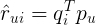
\includegraphics[]{/recommender/predictrating.png}
     \caption{How a prediction for a rating is calculated}
     \label{fig:predictrating}
 \end{figure}
 \noindent
To learn the factor vectors $p_{u}$ and $q_{i}$ used for the equation in \autoref{fig:predictrating}, the recommender system minimizes the squared error of the set of known ratings, that is, the entries in the ratings matrix that have a value:
 \begin{figure}[H]
    \centering
    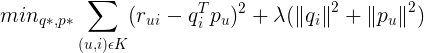
\includegraphics{/recommender/minimizesquarederror.png}
     \caption{How to calculate the squared error once predictions have been made}
     \label{fig:minimizesquarederror}
 \end{figure}
 \noindent
 In \autoref{fig:minimizesquarederror}, $K$ is the set of $(u, i)$ pairs for which the rating $r_{ui}$ is known.
 The system learns by fitting previously observed data, but to avoid overfitting when predicting future ratings, it regularizes the learned parameters.
 This regularization is found on the right side of the $+$ operator of the equation, where $\lambda$ is an arbitrary constant that controls the extent of the regularization.
 Stochastic gradient descent is one approach of minimizing the above equation.
 The algorithm will, in this approach, loop through all data in the training set, which is the currently known ratings.
 For each case, the system predicts a rating, and then computes the prediction error with the equation defined in \autoref{fig:calculatingerror}.
 \begin{figure}[H]
    \centering
    
\includegraphics[]{/recommender/calculatingerror.png}
     \caption{The equation for calculating the error of a prediction when the actual value is known}
     \label{fig:calculatingerror}
 \end{figure}
 \noindent
 After the error has been calculated, the algorithm modifies the parameters through the update rules shown in Figures \ref{fig:updatingq} and \ref{fig:updatingp}.
 \begin{figure}[H]
    \centering
    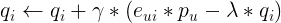
\includegraphics[]{/recommender/updatingq.png}
     \caption{The rule for updating the value of $q$}
     \label{fig:updatingq}
 \end{figure}
 \noindent
 
 \begin{figure}[H]
    \centering
    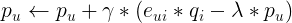
\includegraphics[]{/recommender/updatingp.png}
     \caption{The rule for updating the value of $p$}
     \label{fig:updatingp}
 \end{figure}
 \noindent
 For the update rules, $\gamma$ is the magnitude to which the parameters are modified, and is arbitrary.
 The calculations are performed until the squared error reaches a sufficiently small value, or a max number of iterations has been performed by the algorithm.
 